%MÁSTER UNIVERSITARIO EN GESTIÓN SOSTENIBLE DE LA TIERRA Y EL TERRITORIO
%TÉCNICAS DE ANÁLISIS CUANTITATIVAS Y CUALITATIVAS
%DOCUMENTO DE RESOLUCIÓN DEL EJERCICIO 4 DE EVALUACIÓN
%MARCOS RIAL DOCAMPO


\documentclass[11pt,a4paper]{article}

\usepackage[utf8]{inputenc}
\usepackage[spanish]{babel}
\usepackage{amsmath}
\usepackage{amsfonts}
\usepackage{amssymb}
\usepackage{url}
\usepackage[colorlinks,linktocpage=true,citecolor=blue,linkcolor=blue]{hyperref}
\usepackage{booktabs}
\usepackage{graphicx,geometry}
\usepackage{caption}
\usepackage{verbatim,moreverb}

\usepackage{listings}
\lstset{
	frame=tb,
    framerule=0pt,
    aboveskip=3mm,
    belowskip=3mm,
    framextopmargin=3pt,
    framexbottommargin=3pt,
    %framexleftmargin=0.2cm,
    framesep=0pt,
    rulesep=.4pt,
    backgroundcolor=\color{gray97},
    rulesepcolor=\color{black},
    stringstyle=\color{mauve},
    showstringspaces = false,
    basicstyle=\footnotesize\ttfamily,
    commentstyle=\color{dkgreen},
    keywordstyle=\color{blue},
    numbers=left,
    numbersep=-6.5pt,
    numberstyle=\tiny\color{gray},
    numberfirstline = false,
    breaklines=true,
    morekeywords={*,...}
   }

\usepackage{xcolor}
\definecolor{gray97}{gray}{.97}
\definecolor{gray75}{gray}{.75}
\definecolor{gray45}{gray}{.45}
\definecolor{mauve}{rgb}{0.58,0,0.82}
\definecolor{dkgreen}{rgb}{0,0.6,0}

\author{Marcos Rial Docampo}
\title{Técnicas de Análisis Cuantitativas y Cualitativas\\Resolución del ejercicio de evaluación 4}
\date{\small{\today}}

\begin{document}
\maketitle

Disponemos de datos de los tiempos obtenidos por los participantes de una carrera popular. Se trata de 80 muestras de un total de 1140 que están estratificadas por sexo y categoría de edad.

Mediante un test de Shapiro-Wilk comprobamos si la variable \textit{total.minutos} tiene una distribución normal. Para ello podemos aplicar el test a todas las observaciones de la variable o dividirla en grupos. En este caso dividiremos la variable en los siente grupos correspondientes a la categoría de la prueba, pero podríamos haberlo hecho por sexo o por subcategoría. Obtenemos los resultados mostrados en el cuadro \ref{tab:Shapiro} y los gráficos de la figura \ref{fig:diagrama}.

\begin{table}[ht]
\centering
\begin{tabular}{cr@{,}lr@{,}l}
\toprule[0.4mm]
\multicolumn{5}{c}{Test Shapiro-Wilk}\\
 & \multicolumn{2}{c}{W} & \multicolumn{2}{c}{p-valor}\\
\midrule
Infantil-Cadete & 0&93455 & 0&1888\\
Junior & 0&93301 & 0&1765\\
Senior & 0&96890 & 0&7315\\
Veterano & 0&96757 & 0&7029\\
\bottomrule[0.4mm]
\end{tabular}
\captionsetup{font={footnotesize,it}}
\caption{Resultado del test de Shapiro-Wilk para la variable \textit{total.minutos}.}
\label{tab:Shapiro}
\end{table}

\begin{figure}
\centering
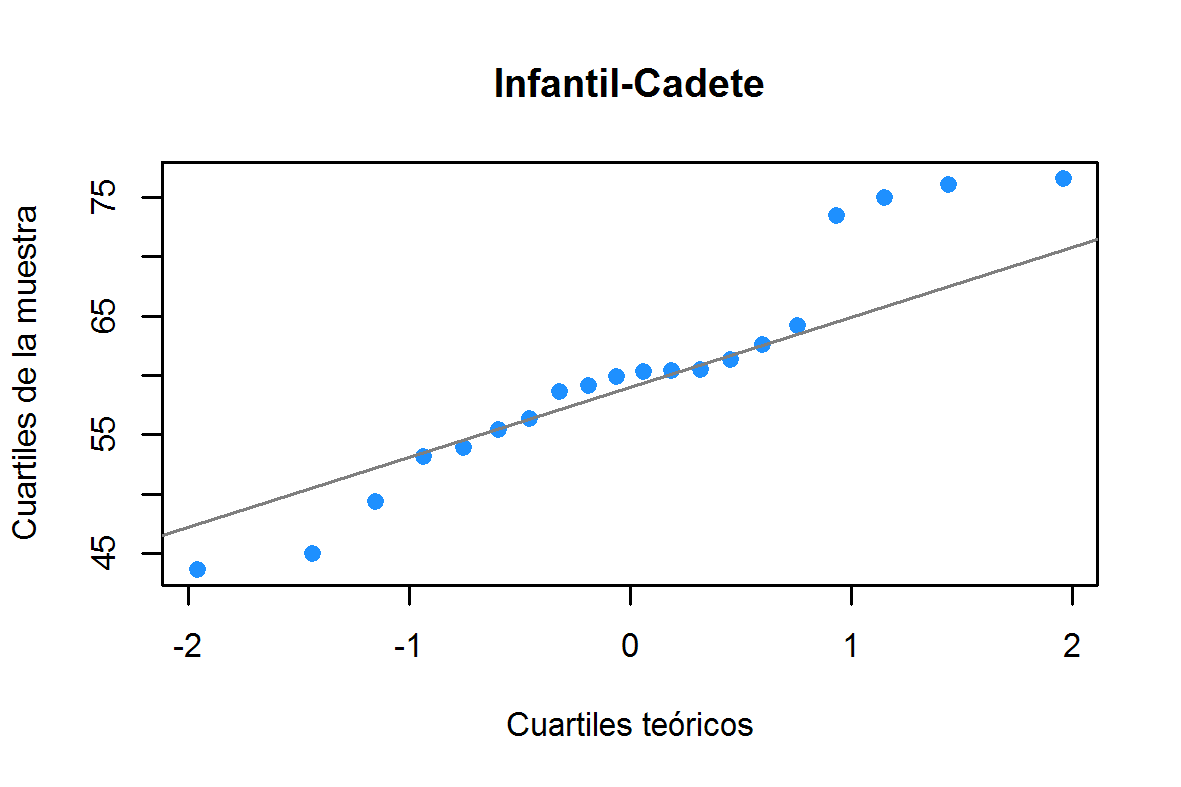
\includegraphics[scale=0.725]{./R/Graficos/CuartInfantil.png}
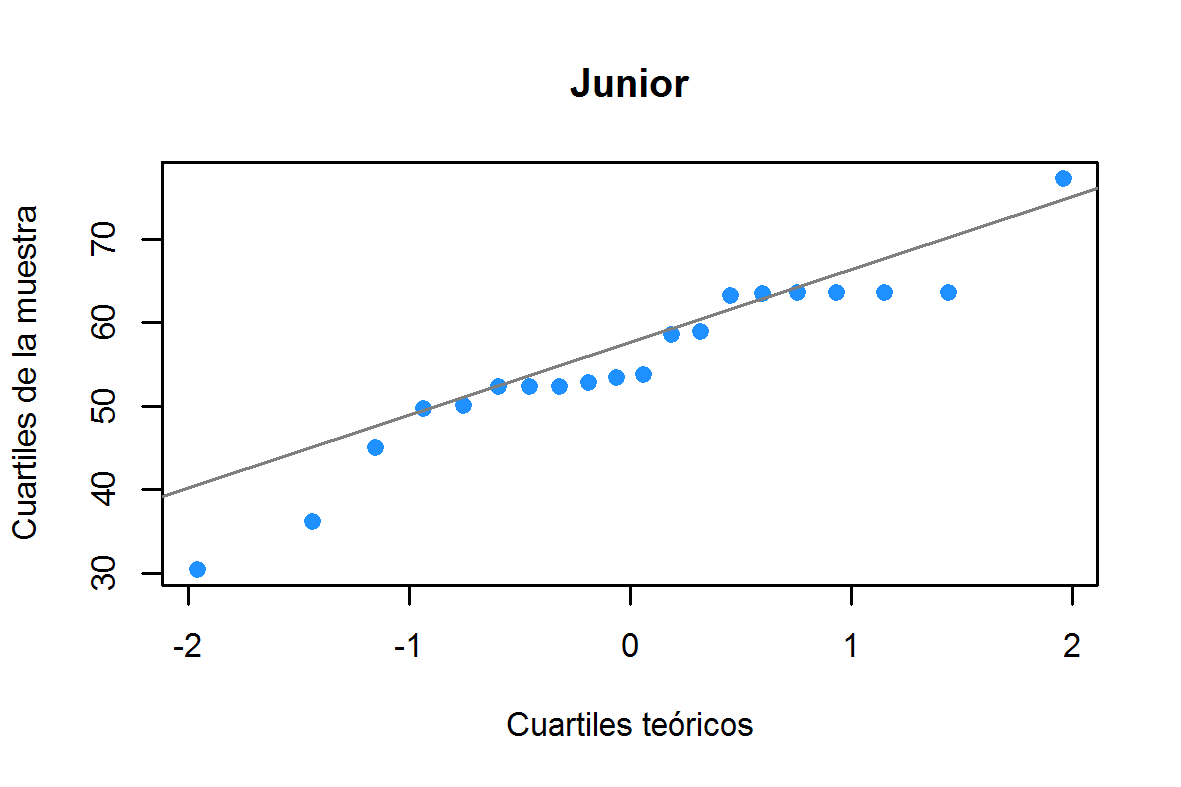
\includegraphics[scale=0.725]{./R/Graficos/CuartJunior.png}
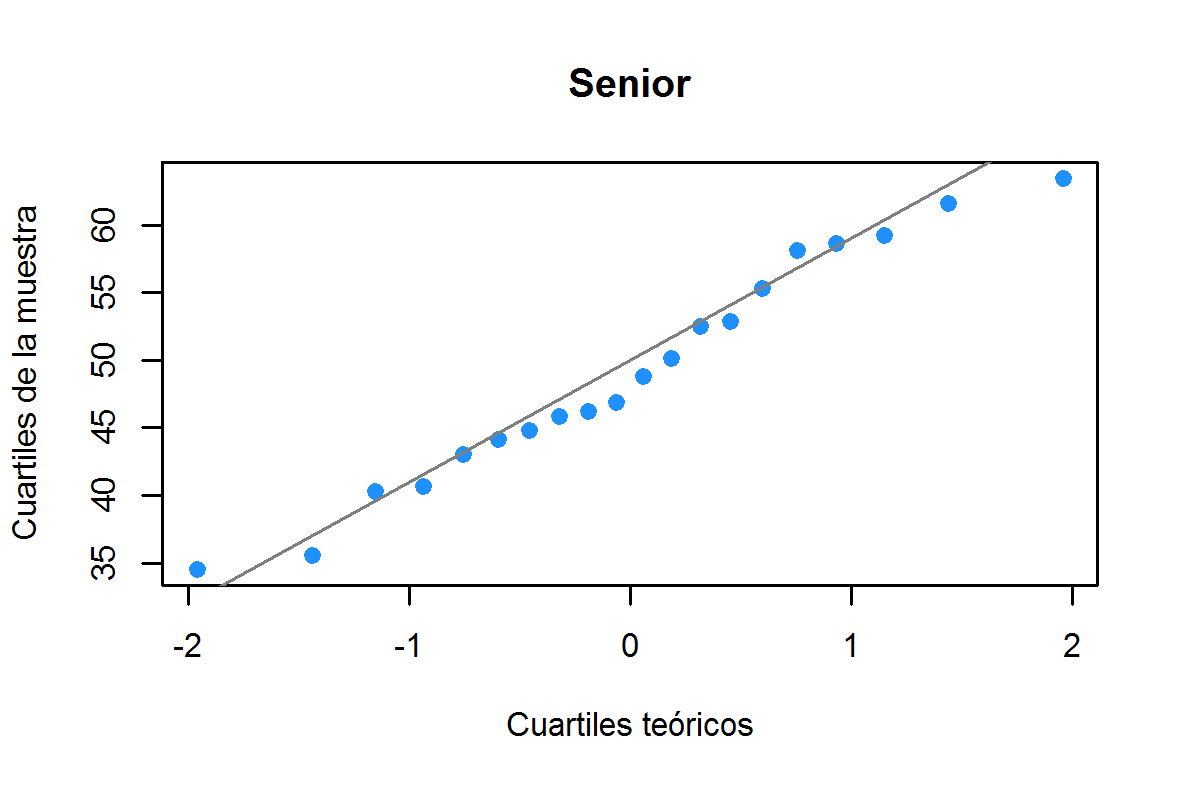
\includegraphics[scale=0.725]{./R/Graficos/CuartSenior.png}
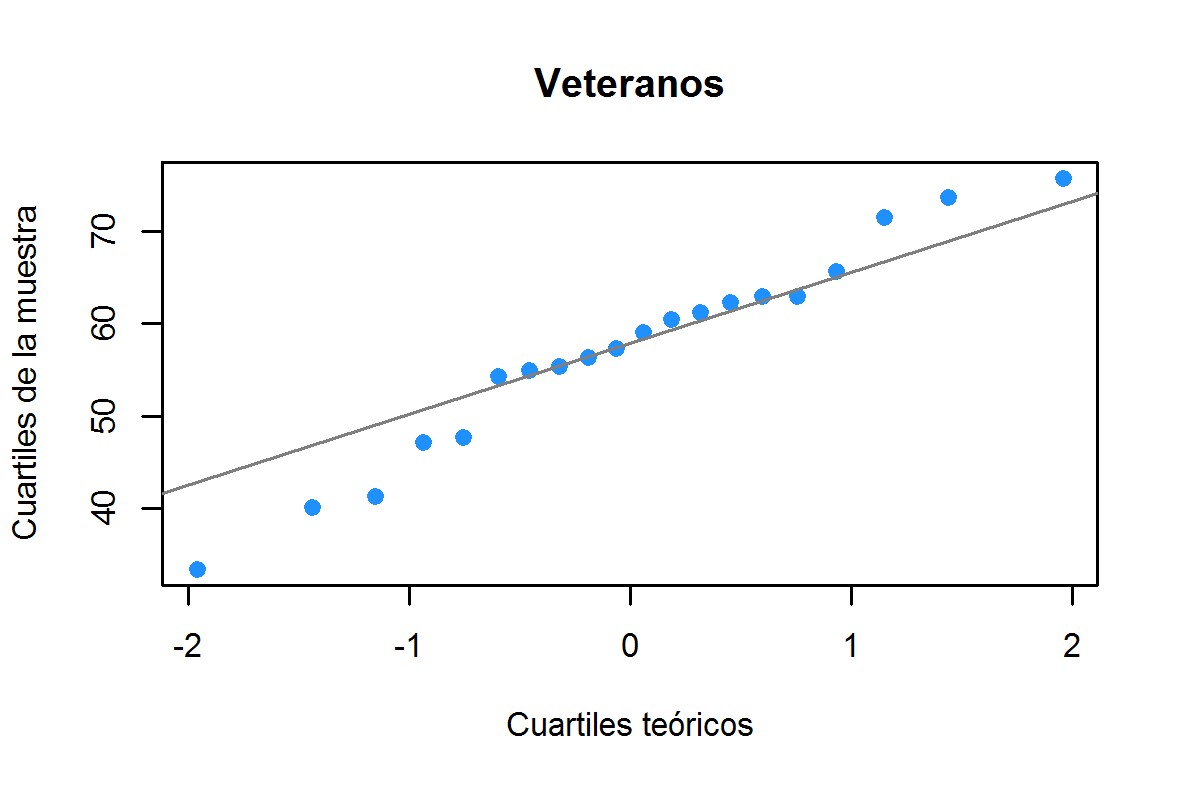
\includegraphics[scale=0.725]{./R/Graficos/CuartVeteranos.png}
\captionsetup{font={footnotesize,it}}
\caption{Diagramas de cuartiles para las categorías de la muestra.}
\label{fig:diagrama}
\end{figure}

\end{document}